% Created 2018-09-30 Sun 23:10
% Intended LaTeX compiler: pdflatex
\documentclass[10pt,t]{beamer}
\usepackage[utf8]{inputenc}
\usepackage[T1]{fontenc}
\usepackage{graphicx}
\usepackage{grffile}
\usepackage{longtable}
\usepackage{wrapfig}
\usepackage{rotating}
\usepackage[normalem]{ulem}
\usepackage{amsmath}
\usepackage{textcomp}
\usepackage{amssymb}
\usepackage{capt-of}
\usepackage{hyperref}
\usetheme{default}
\author{L. Larrabee Strow}
\date{\today}
\title{\large A Long-Term Homogeneous Hyperspectral Radiance Time Series: AIRS2CrIS}
\date{\textit{\footnotesize June 20, 2018}}
\input beamer_setup
\usetheme{metropolis}
\metroset{titleformat title=allcaps}
\renewcommand{\UrlFont}{\small\tt}
\renewcommand*{\UrlFont}{\footnotesize}
\tolerance=1000
\RequirePackage{fancyvrb}
\DefineVerbatimEnvironment{verbatim}{Verbatim}{fontsize=\footnotesize}
\author{L.~Larrabee~Strow and Howard~Motteler (UMBC)}
\hypersetup{
 pdfauthor={L. Larrabee Strow},
 pdftitle={\large A Long-Term Homogeneous Hyperspectral Radiance Time Series: AIRS2CrIS},
 pdfkeywords={},
 pdfsubject={},
 pdfcreator={Emacs 25.3.1 (Org mode 9.1.12)}, 
 pdflang={English}}
\begin{document}

\maketitle
\addtobeamertemplate{block begin}{
  \setlength{\parsep}{0pt}
  \setlength{\topsep}{3pt plus 2pt minus 2.5pt}
  \setlength{\itemsep}{0pt plus 0pt minus 2pt}
  \setlength{\partopsep}{2pt}
}

\begin{frame}[label={sec:org52d7519}]{Introduction}
\vspace{-0.2in}
\begin{center}
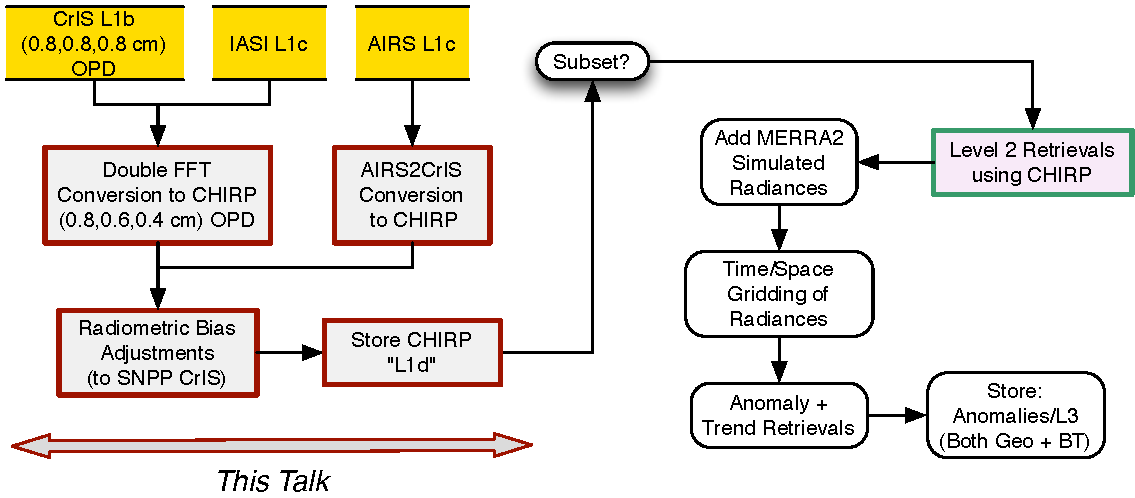
\includegraphics[width=1.0\linewidth]{./Figs/Pdf/airs2cris_stm_talk1_landscape.pdf}
\end{center}

\begin{block}{CHIRP: (Common or Climate) Hyperspectral InfraRed Product}
\begin{description}
\item[{OPD:}] 0.8 / 0.6 /0.4 cm
\item[{Spectral Spacing:}] 0.0625 / 0.0833 / 0.1250 \wn
\end{description}
\end{block}
\end{frame}

\begin{frame}[shrink=5,label={sec:orgd1ba206}]{Why CHIRP}
\vspace{-0.2in}

\begin{itemize}
\item Convert AIRS, CrIS, IASI to a common spectral spectral response function
(SRF)
\item Correct for instrumental radiance offsets
\item Provides long-term radiance continuity over different instruments
\item Allows use of a single forward model (Radiative Transfer Algorithm) for
retrievals
\item Common SRF for AIRS/CrIS and IASI (1:30 and 9:30 equator crossings)
\item Applications
\begin{itemize}
\item Gridded (time/space) radiance products (“L1G”)
\item Geophysical retrievals (anomalies, trends) directly from all-sky radiance  anomaly/trends.  (See talk by L. Strow)
\end{itemize}
\item OLR trends directly from radiance trend retrievals (See talk by Sergio
DeSouza-Machado)
\item Use for Level 2 retrievals?  Only way to mitigate radiance calibration
difference among instruments and to achieve common sensitivity (both for
radiances and RTA)
\end{itemize}
\end{frame}






\begin{frame}[label={sec:orgcb7f6ca}]{CHIRP Data Flow}
\vspace{-0.1in}

\begin{center}
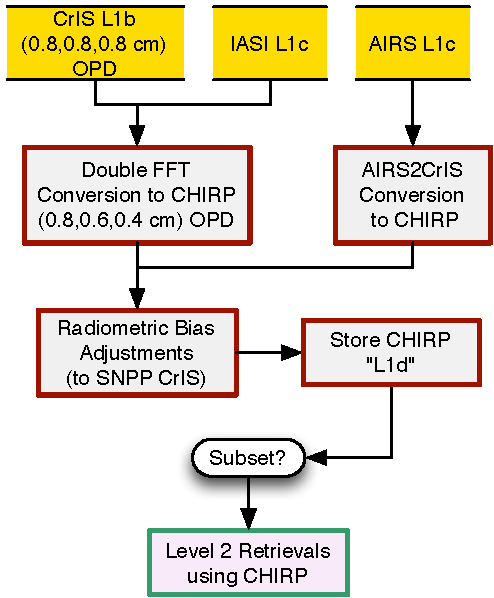
\includegraphics[width=0.6\linewidth]{./Figs/Pdf/airs2cris_stm_talk1_small.pdf}
\end{center}
\end{frame}
\end{document}